\begin{figure}
\begin{center}
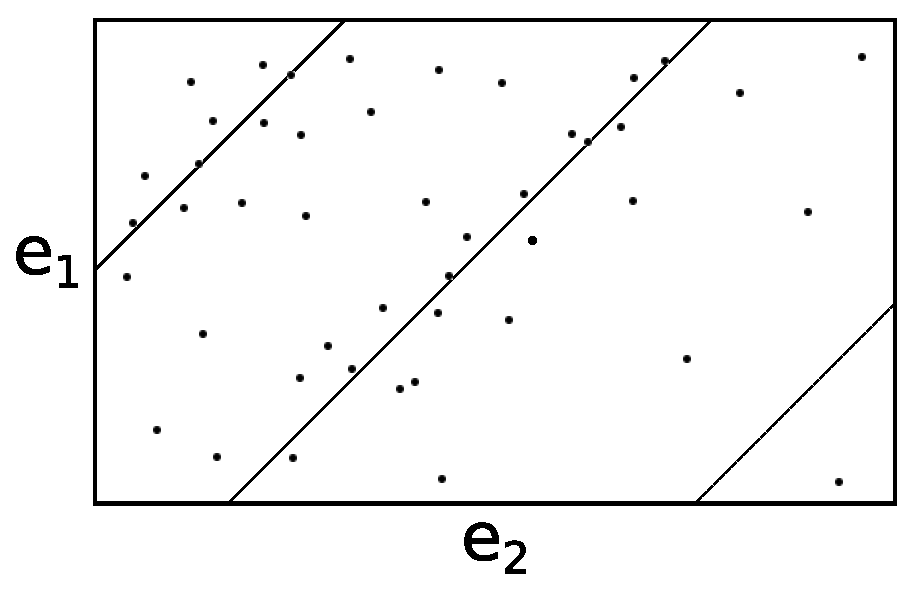
\includegraphics[scale=0.5]{fig/rectangle.eps}
\caption{Example of rectangle with three diagonals. Rightmost diagonal isn't well supported my mate pairs, while other two are well supported. The point which is observed in the lower right corner could appear because of chimeric mate pairs or sequencing errors.}
\end{center}
\end{figure}


\section{Results}

\textbf{Assembly datasets}
%
We used three datasets from \cite{Chitsaz2011}.
A single {\ecoli} cell
and a single marine cell ({\em Deltaproteobacterum} SAR324)
were isolated by micromanipulation as described in \cite{Ishoey2008}.
Paired-end libraries were generated on an Illumina Genome Analyzer IIx from MDA-amplified single-cell DNA
and
from standard (multicell) genomic DNA prepared from cultured {\ecoli}.

We call these datasets SAR324, ECOLI-SC, and ECOLI-MC.
ECOLI-SC and ECOLI-MC are called ``{\ecoli} lane 1'' and ``{\ecoli} lane normal'' in \cite{Chitsaz2011}.
They consist of 100 bp paired-end reads
with average insert sizes 266 bp for ECOLI-SC, 215 bp for ECOLI-MC,
and 240 bp for SAR324.
Both datasets have $600\times$ coverage.

\textbf{Benchmarking}

We benchmarked seven assemblers
(EULER-SR \cite{Chaisson08}, IDBA \cite{Peng10}, SOAPdenovo \cite{Li10}, Velvet \cite{Zerbino08}, Velvet-SC \cite{Chitsaz2011}, E+V-SC \cite{Chitsaz2011} and {\spades}) on three datasets
(ECOLI-SC, ECOLI-MC, and SAR324). To provide unbiased
benchmarking, we used the assembly evaluation tool Plantagora \cite{Barthelson2011}. See Table \ref{Table1}.

{\spades}-rectangle shows improvement over previous SPAdes algorithms. In ECOLI-MC dataset {\spades}-rectangle produce larger N50, almost the same largest contig and the same number of misasseblies.

Improvement is even more significant for single-cell dataset which can be explained by the fact that {\spades}-rectangle better determine and utilize correct distance between edges in the de Bruin graph given datasets with highly uneven coverage. {\spades}-rectangle procudes higher N50 (56,842 bp vs 49,623 by {\spades}), higher largest contig (209,690 bp vs 177,944 by {\spades}), no misassemblies and also captures 64 additional genes (3975 vs 3911 by {\spades}). All other assemblers except of {\spades} and {\spades}-rectangle produced below average results on the single-cell dataset.

Most important that on all datasets {\spades}-rectangle was able to capture more genes than any previous assemblers including {\spades}. New genes are most important in study of new species that cannot be sequenced by classical multi-cell approach.

We further compared E+V-SC, {\spades} and {\spades}-rectangle on the SAR324 dataset.
{\spades}-rectangle assembled contigs totaling ????? bp
(vs. 5,129,304 bp for {\spades} and 4,255,983 bp for E+V-SC) and an N50 of ????? bp (as compared to 75,366 bp for {\spades} and 30,293 bp for E+V-SC).
Since the complete genome of \emph{Deltaproteobacterium} SAR324 is unknown,
we used {\em long ORFs} to estimate the number of genes longer than 600 bp, as a proxy for assembly quality (see \cite{Chitsaz2011}).
There are ???? long ORFs in the {\spades}-rectangle assembly
vs. 2603 for {\spades} and 2377 for E+V-SC.
% I forgot to run on SAR324, doing it now.

  %\def\ra#1{\rotatebox{90}{\parbox{1.0in}{#1}}}
  \def\mrk#1{{\bf #1}}


  %%%%%%%%%%%%%%%%%%%%%%%%%%%%%%%%%%%%%%%%%%%%%%%%%%
  % Table notes, adapted from PNAS
  \newcount\tablenoteloopnum
  \newcount\tablenotenum

  \makeatletter
  \def\tablenote#1{\global\advance\tablenotenum by 1\relax
  $^{\@alph{\the\tablenotenum}}$\expandafter\gdef\csname 
  tabnote\the\tablenotenum\endcsname{#1}}

  \def\tablenotes{\tablenoteloopnum=\tablenotenum
  \global\advance\tablenoteloopnum by 1
  \tablenotenum=0
  {\footnotesize
  \leftskip=0pt \rightskip=\leftskip
  \parfillskip=0pt plus 1 fil
  \loop
  \vskip2pt
  \noindent
  \global\advance\tablenotenum by 1
  \ifnum\tablenotenum<\tablenoteloopnum
  $^{\@alph{\the\tablenotenum}}$\csname 
  tabnote\the\tablenotenum\endcsname
  \repeat}
  }
  \makeatother
  %%%%%%%%%%%%%%%%%%%%%%%%%%%%%%%%%%%%%%%%%%%%%%%%%%

  \begin{table}
  \small

  \caption{
  %\textbf{Table~1.
  Comparison of assemblies
  for
  single-cell (ECOLI-SC) and
  standard
  (ECOLI-MC) datasets.
  }\label{Table1}


  %\vspace*{-0.2in}

  \tabcolsep=4pt
  %\rowcolors{1}{}{lightgray}
  \begin{tabular}{@{\extracolsep{1pt}}p{.2in}p{1.1in}rrrrrrrr}
  %\begin{tabular*}{\hsize}{@{\extracolsep{\fill}}p{.2in}p{1.1in}rrrrrrrr}
  %\begin{tabular}{p{.2in}p{1.1in}rrrrrrrrr}
  %\toprule
   &
      Assembler%
      \tablenote{%
        The best assembler by each criteria is
        indicated in bold. EULER-SR 2.0.1, Velvet 0.7.60, Velvet-SC, and
        E+V-SC were run with vertex size 55.
        %equal to 55.
        %Edena 2.1.1 49 was run with a minimum overlap of 55.
        SOAPdenovo 1.0.4 was run
        with vertex size 27--31. IDBA was run in its default iterative mode;
        IDBA crashed on ECOLI-SC, so IDBA results are only shown for ECOLI-MC.
        {\spades}-single refers to {\spades} without Stages 2 and 3,
        %(without using read-pair information)
        for
  %       an unbiased 
         comparison with E+V-SC, which does not use read-pair information.
        {\spades}, {\spades}-single and {\spades}-rectangle iterated over 
        %vertex sizes 21, 33, 55 (
        edge sizes $k=22,34,56$.
        %{\ecoli} gene annotations
        %were from http://www.ecogene.org/\;.
         Statistics in this table differ slightly from statistics presented in~\cite{Chitsaz2011}
         due to the specific criteria used in Plantagora.
       %  \glenn{Alexey et al: It's not just the number of misassemblies that changed.  Also substitution error rate changed (why?) and number of complete and partial genes changed.  Are you using the same set of annotated genes that I gave you that were used in the Chitsaz et al paper, or a different set?  Do you show all contigs, or do you filter out contigs below a certain size (110 bp was used in Chitsaz et al, 200 bp is used in HMP consortium).  Please at least explain it by email; we need to be prepared to explain this discrepancy if a referee asks.}
  %       since Plantagora has a strict criteria for misassemblies.
        % \glenn{There are differences in substitution error rate and numbers of complete and partial genes as well.  Is the SP lab using a different set of annotated genes?  Different small contig size cutoff?  Etc.  We have to change this explanation.}
      }
   & \# contigs
   & N50~(bp)
   & Largest~(bp)%
    \tablenote{Length of the largest contig without a misassembly.}
   & Total~(bp)%
          \tablenote{The total assembly size may increase (and in some cases exceeds the
           genome size) due to contaminants (see~\cite{Chitsaz2011}),
           misassembled contigs, repeats, and hubs that contribute to multiple contigs.
           The percentage of the {\ecoli} genome covered filters out these issues.
           %Since our datasets include contaminant reads (see~\cite{Chitsaz2011}),
           % for details),
           %the total assembly size may exceed the genome size.
          }
   & Covered (\%)%
         \tablenote{\emph{Percent of genome covered} is the ratio of total number of aligned bases in the assembly to the genome size.
         %This may shrink from the total assembly size due to assembly of contaminants.
  %       However, it may also increase due to small contigs that align to multiple places.
  %       (which are counted with multiplicity by Nucmer).
  %       Note that some small contigs may align to multiple places in the genome, and thus
  %       increase the percent of genome covered.
       %  \glenn{Alexey needs to add a brief description earlier of how we used Plantagora, MAUVE, and Nucmer, and citations for all three, not just Plantagora.}
         }
   & MA%Misassemblies%
         \tablenote{MA: \emph{Misassemblies} are locations on an assembled contig where the left flanking sequence aligns over 1~kb away from the right flanking sequence on the reference.}
   & MM%Mismatches (per 100 kbp)%
         \tablenote{MM: Mismatch (substitution) error rate per 100 kbp is measured in the correctly assembled contigs.}
   & CG%Complete genes%\\
         \tablenote{CG: Complete genes out of 4,324 genes annotated at http://www.ecogene.org\;.}
   %(among 4324 known)
  % & \ra{Complete plus \\ partial genes%
  %       \tablenote{
  %         ``Partial genes'' are genes with an overlap of at least 100 nucleotides
  %         with a contig, but not wholly contained in the contig;
  %         see~\cite{Chitsaz2011}.
           %``Partial genes'' are defined as in~\cite{Chitsaz2011}.
           %A gene is ``partially'' present in the assembly if it has an overlap
           %of at least 100 nucleotides with a contig, but is not completely
           %contained in the contig.
  %       }
  %   }
   \\
     \hline
  %\midrule
  %\smallskip
  \\[-6pt]
  \multicolumn{10}{l}{\bf Single-cell {\ecoli} (ECOLI-SC)}\\
  %\\[-9pt]
   & EULER-SR                 &      1344 &           26662 &                       126616 &    4369634 &         87.8 &            21 &                     11.0 &                   3457 \\%&         3889 \\
  %& Edena                    &      1592 &            3919 &                        44031 &    3996911 &         79.1 &            12 &                      2.1 &                   2440 &         3569 \\
   & SOAPdenovo               &      1240 &           18468 &                        87533 &    4237595 &         82.5 &            13 &                     99.5 &                   3059 \\%&         3653 \\
   & Velvet                   & \mrk{428} &           22648 &                       132865 &    3533351 &         75.8 &             2 &                \mrk{1.9} &                   3117 \\%&         3288 \\
   & Velvet-SC                &       872 &           19791 &                       121367 &    4589603 &         93.8 &             2 &                      \mrk{1.9} &                   3654 \\%&         4010 \\
   & E+V-SC                     &       501 &           32051 &                       132865 &    4570583 &         93.8 &             2 &                      6.7 &                   3809 \\%&         4001 \\
    & {\spades}-single               &      1164 &           42492 &                       166117 &    4781576 &   \mrk{96.1}  &       1 &                      6.2 &                   3888 \\%&   \mrk{4177} \\
   & {\spades}                   &      1024 &     49623 &                 177944 &    4790509 &         \mrk{96.1} &       1 &                      5.2 &             3911 \\ %&         4172 \\[3pt]
   & {\spades}-rectangle                   &      509 &     \mrk{56842} &                 \mrk{209690} &    4550761 &         95.5 &       \mrk{0} &                      3.6 &             \mrk{3975} \\[9pt] %&         4172 \\[3pt]
   %
  %
  % & {\spades}-single reads               &      1241 &           38138 &                       133927 &    4621694 &   \mrk{96.12}%
  %\tablenote{A manual analysis revealed that a  212 bp contig marked as misassembled by {\spades}-single is actually a Plantagora alignment artifact.
  %% rather than misasembly.
  %}
  %  &             1 &                      3.3 &                   3879 &   \mrk{4179} \\
  % & {\spades}                   &       845 &     \mrk{45436} &                 \mrk{209370} &    4633764 &         95.65 &       \mrk{0} &                      5.5 &             \mrk{3892} &         4158 \\[3pt]
  \multicolumn{10}{l}{\bf Normal multicell sample of {\ecoli} (ECOLI-MC)}\\
  %\\[-9pt]
   & EULER-SR                           &       295 &    \mrk{110153} &            221409 &    4598020 &        99.5 &            10 &                      5.2 &                  4232 \\%&         4306 \\
  %& Edena                              &      1673 &            3814 &             20470 &    4611645 &        97.0 &             6 &                      2.8 &                  3020 &         4212 \\
  & IDBA                               & \mrk{191} &           50818 &            164392 &    4566786 &        99.5 &             4 &                      1.0 &                  4201 \\%&         4314 \\
   & SOAPdenovo                         &       192 &           62512 &            172567 &    4529677 &        97.7 &             1 &                     26.1 &                  4141 \\%&         4220 \\
   & Velvet                             &       198 &           78602 &      196677 &    4570131 &       \mrk{99.9} &             4 &                1.2 &                  4223 \\%&         4309 \\
   & Velvet-SC                          &       350 &           52522 &            166115 &    4571760 &        \mrk{99.9} &       \mrk{0} &                      1.3 &                  4165 \\%&         4265 \\
   & E+V-SC                             &       339 &           54856 &            166115 &    4571406 &        \mrk{99.9} &       \mrk{0} &                      2.9 &                  4172 \\%&         4264 \\
   & {\spades}-single                         &       445 &           59666 &            166117 &    4578486 & \mrk{99.9} &       \mrk{0} &                     \mrk{0.7} &                  4246 \\%&   \mrk{4317} \\
   & {\spades}                             &       195 &           86590 &            \mrk{222950} &    4608505  &   \mrk{99.9}  &             2 &                      3.7 &             4268 \\%&    \mrk{4318} \\
   & {\spades}-rectangle                   &      192 &     91893 &                 221829 &    4593658 &         \mrk{99.9} &       2 &                      3.5 &             \mrk{4274} \\ %&         
   & Velvet-IDEAL                   &      296 &     95398 &                 269661 &    4566339 &         \mrk{99.85} &       0 &                      ??? &             \mrk{4267} \\ %&         
   \hline
  %\bottomrule
  \end{tabular}

  \bigskip

  \tablenotes

  %\bigskip


  %\vspace*{-0.2in}

  \end{table}


\textbf{Running time and memory requirements}

SPAdes memory and time complexity were analysed in \cite{SPAdes}. Most time and memory consuming stages in genome assembly are, usually, de Bruijn graph construction and mapping reads to edges. After this stages are done, repeat resolution routine can work relatively fast and within small memory.

For both {\ecoli} datasets and SAR324, our rectangle approach works for less then 10 seconds given (1) unresolved de Bruijn graph from SPAdes-single and (2) mapping positions of all mate-pair reads to the graph. All datasets where analysed using less than 100 MB RAM.
